\section{Revisión de antecedentes}
\subsection{Clasificación de escenas mediante Redes Neuronales Recurrentes}
En \cite{lstm_real_estate} J. H. Bappy y otros introducen un framework para aprender la información de las escenas de manera secuencial. Además, generan y hacen público un dataset de aproximadamente 6000 imágenes etiquetadas pertenecientes a las seis partes que consideran más importantes a clasificar de una casa: frente, patio, dormitorio, baño, living y cocina.

Para empezar con la estructura que proponen, es necesario explicar el algoritmo de preprocesamiento que aplican a cada imagen con el fin de intensificar los contrastes locales de la misma. Se trata de una de las variantes de ecualización de histograma de las imágenes llamada Ecualización de Histograma Adaptativo con Limitación de Contraste (o por sus siglas en inglés C.L.A.H.E., Contrast Limited Adaptive Histogram Equalization). Este algoritmo es la evolución de HE (Histogram Equalization) y de AHE (Adaptive Histogram Equalization). 
La Ecualización del Histograma de la imagen incrementa el contraste global de las mismas, sobretodo cuando los datos representativos de la imagen están representados por valores de contraste cercanos.
Por otro lado, la Ecualización del Histograma Adaptativo computa múltiples histogramas correspondientes a diferentes secciones de la imagen, utilizándolos para redistribuir la limunosidad de la misma. La principal mejora es que obtiene mejores contrastes en sectores locales de la imagen, y define mejor límites dentro de cada región.
Este método tiende a amplificar por demás el ruido en regiones relativamente homogéneas de la imagen, la Ecualización del Histograma Adaptativo con Limitación de Contraste se encarga de prevenir esta situación limitando la amplificación, podemos observar un ejemplo de aplicación de esta técnica en la Fig. \ref{fig:lstmclaheexample}.
\begin{figure}[h]
	\centering
	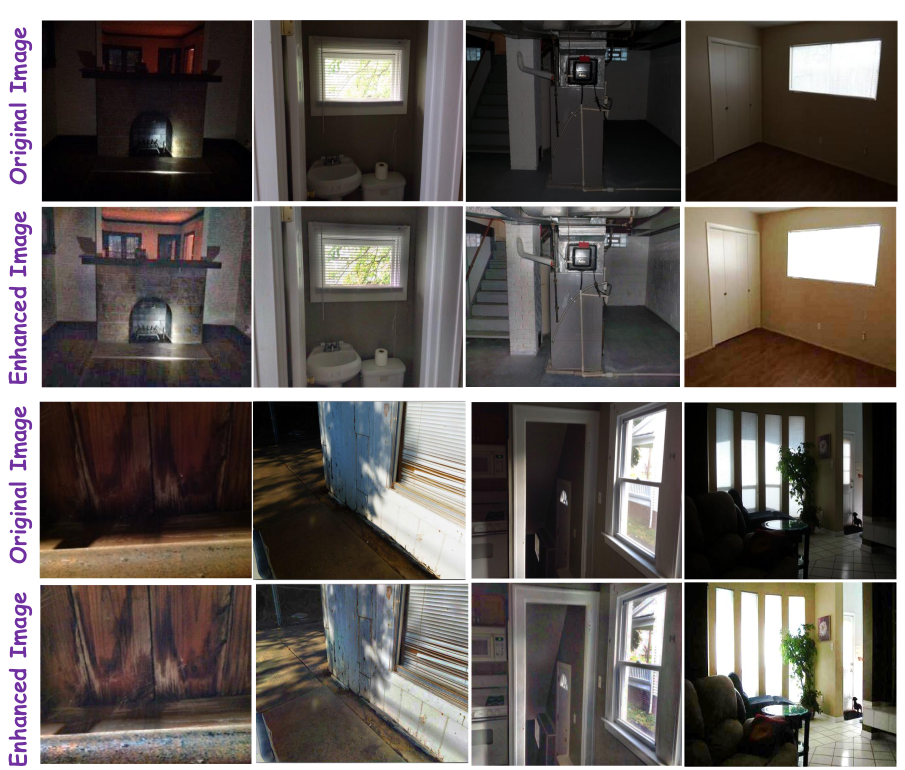
\includegraphics[width=1\linewidth, height=0.5\textheight]{images/lstm_clahe_example}
	\caption[Ejemplo aplicación del algoritmo C.L.A.H.E.]{Ejemplo aplicación del algoritmo C.L.A.H.E.}
	\label{fig:lstmclaheexample}
\end{figure}
La propuesta de estos investigadores se basa en aprender la información de la escena secuencialmente, tanto de forma vertical como horizontal. Para hacerlo, crearon dos redes recurrentes LSTM (Long Short Term Memory) con cuatro (4) capas ocultas de cientoveintiocho (128) unidades cada una. Como segundo punto, alimentan a la red con los datos de las imágenes de forma secuencial, es decir, transforman las imágenes a un tamaño de 128x128 y luego alimentan la red con la información secuencial de cada pixel de forma vertical para una de las redes y de forma horizontal para la otra. Para finalizar, introducen una capa densa totalmente conectada (fully connected layer, en inglés) con las salidas de ambas LSTM, seguida de otra capa densa totalmente conectada que concluye con una capa densa final con activación Softmax.

La arquitectura final propuesta como se puede observar en la Fig. \ref{fig:lstmarchitecture}, queda de la siguiente manera: dos redes LSTM que reciben los pixeles orientados de forma vertical y horizontal, respectivamente; una capa densa totalmente conectada que recibe las salidas de cada celda de la red LSTM, otra capa densa totalmente conectada que se concatena a la anterior y una capa densa final con activación Softmax que brinda las salidas.
Vale mencionar que es necesaria la aplicación del algoritmo CLAHE a cada imagen para el posterior entrenamiento y clasificación mediante la red propuesta.

\begin{figure}[h]
	\centering
	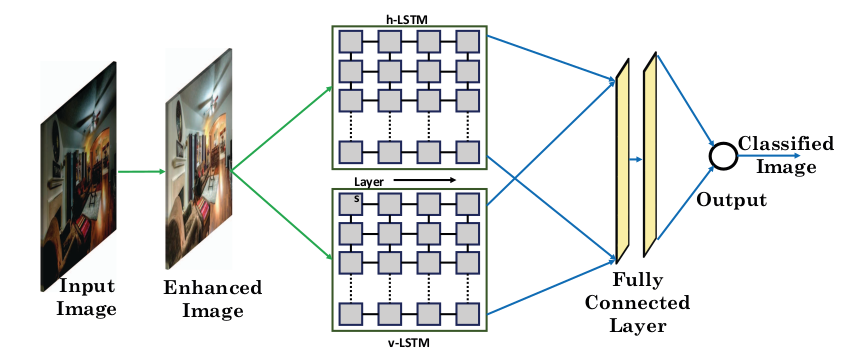
\includegraphics[width=1\linewidth,height=0.3\textheight]{images/lstm_architecture}
	\caption[Arquitectura de la red presentada]{Arquitectura de la red presentada}
	\label{fig:lstmarchitecture}
\end{figure}

Las comparaciones realizadas por los investigadores se basan en la métrica Exactitud (Accuracy, en inglés) y se emplean utilizando diferentes configuraciones de esta red, y comparándose con el dataset que ha propuesto (Real Estate Images, en inglés) y el dataset abierto SUN. A modo de remarcarlo, obtienen como mejores valores un 96.92\% de exactitud en el dataset REI, y un 90.24\% en el dataset SUN, utilizando la configuación descripta anteriormente.
De esta manera quedan por encima de los resultados de utilizar extracción de características de redes preentrenadas como AlexNet con el dataset ImageNet y VGGNet con el dataset ImageNet.

 

\subsection{Clasificación de escenas mediante Redes Neuronales Convolucionales}


En \cite{learning_deep_features} se creó un nuevo dataset con siete (7) millones de imágenes de escenas etiquetadas. Zhou y otros utilizaron redes neuronales convolucionales para aprender características profundas sobre las escenas y alcanzar un nuevo estado del arte. Ellos se encargaron de mostrar que las características de más alto nivel aprendidas por redes neuronales profundas en datasets centrados en objetos y a escenas son diferentes: imágenes de objetos no contienen la riqueza y diversidad de informaión visual que brindan las imágenes de escenas y ambientes para poder identificarlos.

Su trabajo comienza por la construcción del dataset: creación de urls a partir de sustantivos y adjetivos relacionados a las escenas, eliminación de los links duplicados y luego de realizada la descarga, la eliminación de imágenes que se encuentren ya en el SUN database. Comparar la calidad del dataset generado en relación a otros de similar magnitud depende no sólo de las imágenes que contengan y sus categorías, sino también de múltiples factores como la variabilidad de las posiciones de la cámara, los estilos de decorado, la ubicación y el tamaño que los objetos ocupan dentro de la imagen, etc. Es razonable asumir que una buena base de datos de imágenes debería ser densa y diversa. La densidad de una medida de concentración de los datos, y una base de datos de imágenes debe serlo ya que para aprender sobre un elemento (en este caso escenas) es necesario que haya alto grado de concentración de ese elemento. La realidad es que la densidad de un dataset no alcanza, ya que si se cuenta con todas imágenes de la misma habitación tendrá una densidad muy alta pero una diversidad muy escaza. La diversidad es una medida relacionada a la cantidad de clases en un dataset. Un dataset de imágenes debe ser diverso porque es necesario que haya tanto múltiples elementos dentro de la base de datos como también variabilidad de enfoques para sus imágenes. Ambas medidas son difíciles de medir en datasets de imágenes.
En este caso, los autores proponen dos medidas: densidad relativa y diversidad relativa. Para la primera los autores asumen que, en el dominio de los datasets de imágenes, una alta densidad es equivalente a que en general las imágenes tienen vecinos similares. Por esta razón para realizar la medición toman una imagen random de un dataset \(A\) (llámese \(a_{1}\)) y una imagen random del segundo dataset B (llámese \(b_{1}\)). Si el set A es más denso que el set \(B\), entonces es más probable que a1 tenga menor distancia a su vecino más cercano que b1. Con esta definición, se tiene que \(A\) es más denso que \(B\) si y sólo si la densidad de  \(A\) dado  \(B\) es mayor que la densidad de \(B\) dado \(A\). 
\begin{equation}
{Den}_{B}(A)=p\left(d\left(a_{1}, a_{2}\right)<d\left(b_{1}, b_{2}\right)\right)
\end{equation}

Esta noción de densidad entre datasets puede aplicarse a múltiples datasets \({A_{1}, \ldots, A_{N}}\):

\begin{equation}
{Den}_{A_{2}, \ldots, A_{N}}\left(A_{1}\right)=p\left(d\left(a_{11}, a_{12}\right)<\min _{i=2: N} d\left(a_{i 1}, a_{i 2}\right)\right)
\end{equation}

 Si de diversidad se trata, existen varias formas de medirla que mayormente se utilizan en biología para conocer la riqueza de un ecosistema. Para este trabajo los investigadores se basaron en el índice Simpson de diversidad que es una medida de qué tan bien están distribuidos los individuos de las diferentes especies en un ecosistema, y está relacionado a la entropía de la distribución de los mismos. Ellos proponen medir la diversidad relativa de dos datasets basándose en la idea de que si dados dos datasets \(A\) y \(B\), entonces \(A\) resultará más diverso si al selecionar aleatoriamente dos imágenes del dataset \(B\) resultan más similares visualmente que seleccionar aleatoriamente dos imágenes del dataset \(A\). De esta manera, la diversidad de \(A\) con respecto a \(B\) puede ser definida como:
 \begin{equation}
 {Div}_{B}(A)=1-p\left(d\left(a_{1}, a_{2}\right)<d\left(b_{1}, b_{2}\right)\right)
 \end{equation}
  donde \(a_{1}\) y \(a_{2}\) pertencen a \(A\) y  \(b_{1}\) y \(b_{2}\) pertenecen a \(B\) y fueron todas las imágenes seleccionadas aleatoriamente. De igual manera a la medida anterior, es posible de ser calculada entre más datasets \({A_{1}, \ldots, A_{N}}\):
  
  \begin{equation}
  {Div}_{A_{2}, \ldots, A_{N}}\left(A_{1}\right)=1-p\left(d\left(a_{11}, a_{12}\right)<\min _{i=2: N} d\left(a_{i 1}, a_{i 2}\right)\right)
  \end{equation}
  
  siendo \(a_{i 1}, a_{i 2} \in A_{i}\) seleccionados aleatoriamente.
  
En el marco de la experimentación realizada para demostrar que las redes aprenden características diferentes según el tipo de dataset que se utilice para entrenarlas los investigadores se quedaron con aproximadamente 2.48 millones de imágenes correspondientes a 205 categorías con un mínimo de cinco mil y un máximo de quince mil imágenes por cada una como set de entrenamiento (al cual se refieren como "dataset Places205"). El set de validación se seleccionó con cien imágenes por escena y el set de test doscientas, alcanzando un total de cuarenta y un mil imágenes entre estas dos últimas particiones. 
Finalizado el entrenamiento, los investigadores comparan las respuestas de unidades de varias capas de la red para entender mejor las diferencias entre ImageNet-CNN y Places-CNN, dos redes que tienen idéntica arquitectura pero que fueron entrenadas con sets de datos creados para diferentes propósitos (objetos y escenas, respectivamente). Las diferencias mayores entre las activaciones se dan a partir de la capa de pooling númuero dos gradualmente hasta la número cinco y también en la capa totalmente conectada número siete, en las que para ImageNet-CNN los campos receptivos se asemejan más a partes de objetos mientras que para Places-CNN en las mismas capas los campos receptivos parecen ser paisajes o estructuras relacionadas a un espacio. 
\begin{figure}[h!]
	\centering
	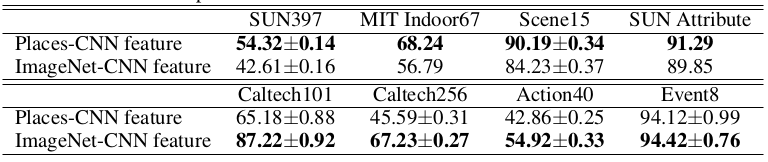
\includegraphics[width=1\linewidth]{images/places_metrics}
	\caption[Métricas por dataset y red]{Métricas por dataset y red}
	\label{fig:placesmetrics}
\end{figure}
En Fig. \ref{fig:placesmetrics} los investigadores hacen una comparación sobre conjuntos de imágenes tanto centradas en objetos como en escenas. La métrica utilizada es exactitud y los sets con que compararon fueron: SUN397, MIT INDOOR67, SCENE15, SUN Attribute, CALTECH101, CALTECH256, ACTION40, EVENT8. En los primeros cuatro, contrados a imágenes, los resultados obtenidos por Places-CNN son mayores a los de ImageNet-CNN. En los segundos cuatro datasets, que son centrados en objetos, ImageNet-CNN es quien comanda en la métrica. 


Para finalizar, entrenaron una red híbrida combinando el set de datos de entrenamiento de Places-CNN y de ImageNet-CNN. La llamaron Hybrid-CNN y luego de remover categorías solapadas alcanzó los 3.5 millones de imágenes pertenecientes a 1183 etiquetas diferentes. Esta red logró pequeñas mejoras en algunos de los datasets utilizados en la comparación entre Places-CNN e ImageNet-CNN. Los resultados se muestran en Fig. \ref{fig:placesmetricshybrid}.
\begin{figure}[h!]
	\centering
	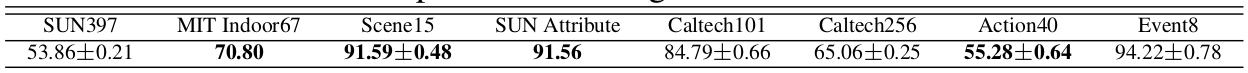
\includegraphics[width=1\linewidth]{images/places_metrics_hybrid}
	\caption[Métricas por dataset - Hybrid-CNN]{Métricas por dataset - Hybrid-CNN}
	\label{fig:placesmetricshybrid}
\end{figure}


En \cite{object_detectors_emerge_in_deep_scene_cnns} demostraron que no es necesario entrenar múltiples redes para realizar las tareas de clasificación de escenas y detección de objetos de una sola vez, ya que los detectores de objetos emergen por sí mismos en redes neuronales convolucionales entrenadas con datasets de escenas. 
Entender las representaciones aprendidas en las capas intermedias de arquitecturas profundas es un factor importante y del cual se podría sacar más provecho. Como las escenas están, en parte, compuestas por objetos, las redes neuronales convolucionales entrenadas para esta tarea aprenden a identificarlos internamente para definir de qué escena se trata, ergo la clasificación de escenas y la detección de objetos puede ser realizada en un mismo recorrido hacia adelante de la red, sin la necesidad de dar a la misma explícitamente la noción de objetos.
La contribución más importante en este trabajo fue demostrar que las redes entrenadas para detección de escenas, internamente aprenden a detectar los objetos relacionados a estas escenas; característica que hace a estas redes explotables para realizar otros propósitos sin la necesidad de tomarse todo el trabajo de crear, entrenar y refinar una red más con la que detectar los objetos que se contienen en estas escenas. En mayor medida, si la red fue entrenada con un dataset centrado en objetos. 
Para esta tarea los investigadores buscaron simplificar las imágenes de entrada para poder conocer cuáles eran las características de éstas que concentraban la mayor parte de la información que utilizada por la red, es decir, aquellas en las que luego de ir quitando resto de características de la escena, la exactitud con la que se predecía se mantenía similar. En el primer intento de realizar esta tarea, para cada imagen, ellos crearon una segmentación a partir de los bordes y regiones, removiendo segmentos en diferentes de la siguiente manera: en cada iteración se remueve aquel segmento que produce el menor decrecimiento en la puntuación de clasificación, hasta que la escena sea clasificada incorrectamente. Al finalizar este primer enfoque obtuvieron una representación de la imagen que contiene la información mínima necesaria para que la red clasifique correctamente la escena. 
En un segundo intento basado en la hipótesis de que para la red Places-CNN existían objetos cruciales en el reconocimiento de escenas, generaron representaciones mínimas de las imágenes anclándose del dataset totalmente anotado SUN Database en cambio de realizar una segmentación automática. Para hacerlo realizaron el mismo procedimiento que en el primer enfoque para obtener estas representaciones con la diferencia que tomaron como verdaderos los segmentos provistos por la base de datos SUN. Vale denotar que para cada escena, son objetos los que usualmente forman parte de la representación mínima necesaria por la red, como es posible observar en la Fig. \ref{fig:objectsdetectorsemergeminrepresentationexamples}.
\begin{figure}[h!]
	\centering
	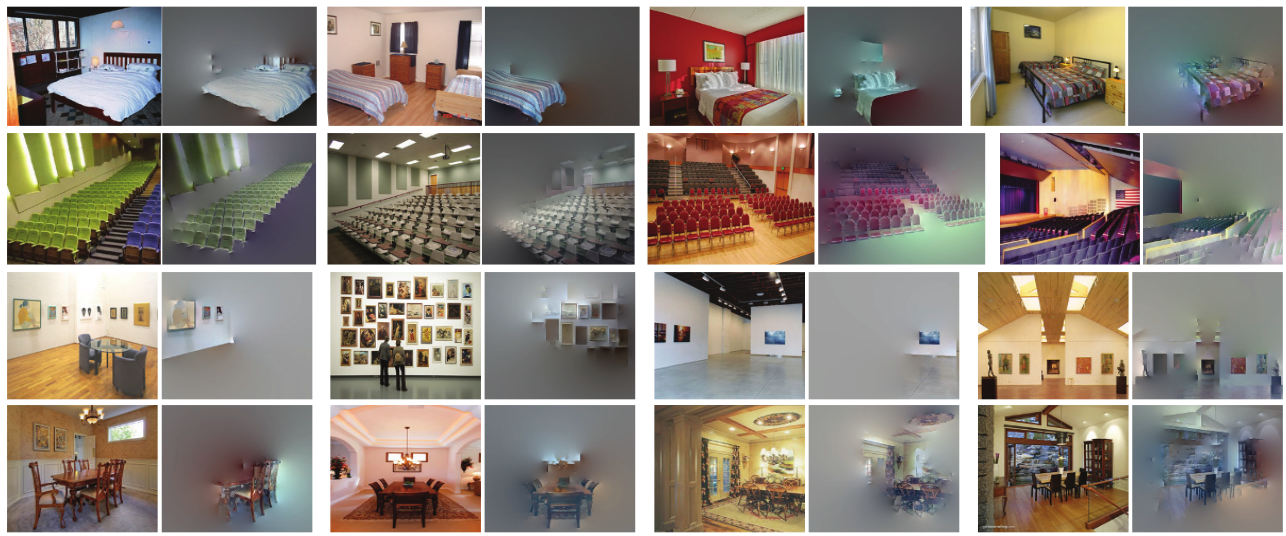
\includegraphics[width=1\linewidth]{images/objects_detectors_emerge_min_representation_examples}
	\caption[Ejemplos de representaciones mínimas encontradas]{Ejemplos de representaciones mínimas encontradas}
	\label{fig:objectsdetectorsemergeminrepresentationexamples}
\end{figure}

Para continuar con el trabajo, realizaron un análisis de los campos receptivos de las unidades y sus patrones de activación. Esto llevó a la observación de que las activaciones de las regiones tienden a tomar en mayor significado semántico a medida que se incrementa en la profundidad de las capas.
Finalmente, los investigadores brindan algunas razones de porqué emergen estos objetos en las tareas de clasificación de escenas: por un lado, que los objetos que emergen son los que más se encontraron en la base de datos SUN, por otro que éstos objetos que emergen son los que permiten discriminar mejor entre diferentes escenas, como es posible de observar en la Fig. 	\ref{fig:objectsdetectorsemergefinalexample}. Gracias a este trabajo es posible alcanzar el estado del arte en clasificación de escenas utilizando la red Places-CNN, pero también aprovechar las capas intermedias para encargarse de detectar los objetos que aparecen en estas escenas a partir de los campos receptivos de las mismas.
\begin{figure}[h!]
	\centering
	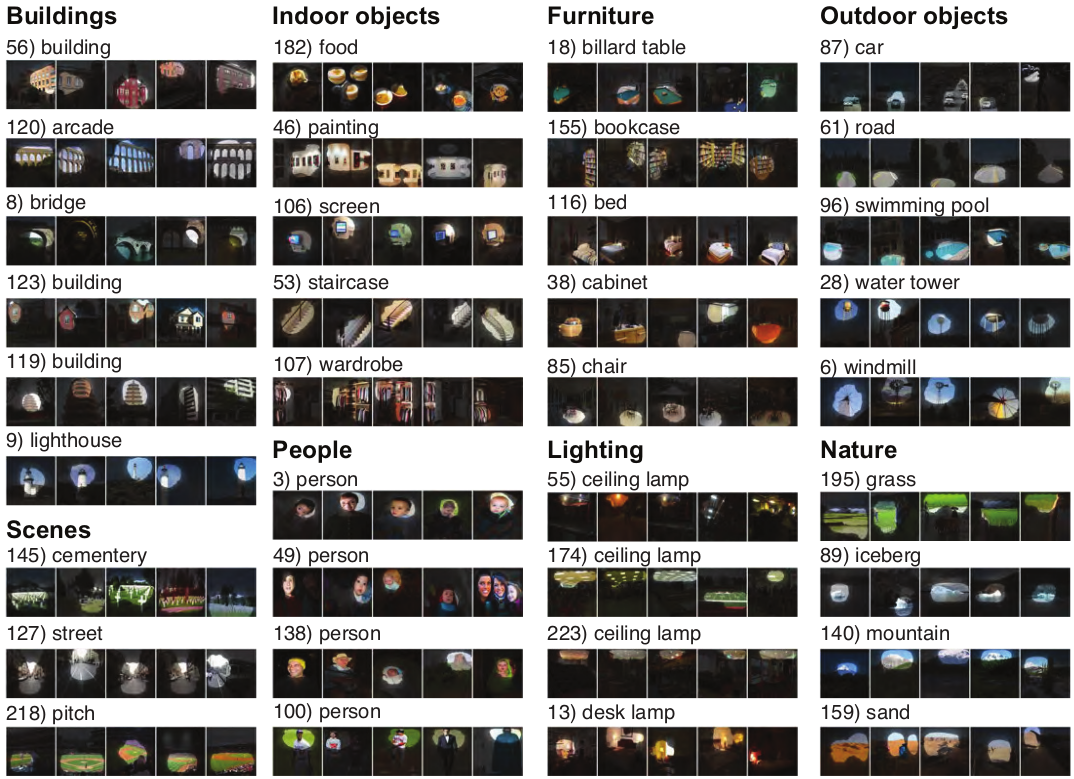
\includegraphics[width=1\linewidth, height=0.7\textheight]{images/objects_detectors_emerge_final_example}
	\caption[Ejemplos de objetos detectados a partir de la capa de pooling número 5]{Ejemplos de objetos detectados a partir de la capa de pooling número 5}
	\label{fig:objectsdetectorsemergefinalexample}
\end{figure}


En \cite{scene_recognition_cnn} Herranz y otros, basándose en la idea de que el reconocimiento de escenas requiere comprender tanto sobre escenas como de objetos en la escena, se dedicaron a la tarea de resolver dos problemas relacionados; por un lado el sesgo inducido por datasets relacionados a objetos de una escala en redes neuronales convolucionales entrenadas con objetos en múltiples escalas y por el otro, cómo combinar eficientemente el conocimiento obtenido de datasets centrados en escenas y de datasets centrados en objetos.

En este trabajo ellos se encargaron de tener en cuenta la escala de los objetos para hacer que la red gane en razón de reconocimiento de las escenas. Para hacerlo eligieron centrarse en dos de los aspectos más importantes de los datasets: escala y densidad. Por el lado de la escala, en el dataset ImageNet cada objeto ocupa casi el total de cada imagen, mientras que por el lado del dataset Sun397 los objetos son mucho más pequeños. Por parte de la densidad, en el dataset centrado en objetos, cada imagen contiene un gran objeto, mientras que en el dataset centrado en escenas cada imagen contiene muchos objetos pequeños.

Gracias a la segmentación de objetos dentro de las escenas que lograron, fueron capaces de crear variaciones de un mismo elemento. De esta manera definieron y generaron los mismos objetos en dos escalas diferentes: escala original (la escala del objeto en la escena original) y escala canónica (se centra el objeto en la imagen y es reescalado para ocupar el tamaño de la imagen, manteniendo aspecto de radio).

La arquitectura propuesta por estos investigadores está enfocada a atender múltiples escalas mediante redes de escalas específicas. Esta gran red es una combinación de varias redes que operan en paralelo sobre sectores extraídos de la versión original de la imagen. Para cada una de las escalas utilizaron una red con una variante de la arquitectura AlexNetCNN llamada Caffe-Net. Para la extracción de los sectores, con el fin de acelerar el procesamiento, utilizaron una red totalmente convolucional (Fully convolutional network), con una capa de agrupamiento mediante máximos para agregar las características de los sectores en características de la imagen en sí.

Ellos detallaron sus dos diferencias principales con la arquitectura híbrida base. Primeramente, ellos utilizan el modelo más adecuado para cada escala de las imágenes. Luego, se encargaron de refinar individualmente los parámetros de cada uno de los modelos generados para adaptarse de la mejor manera a la escala. Además, remarcan que el punto de principal inflexión con el resto de trabajos similares es que ellos le dan importancia a la escala de la imagen, usando varias redes neuronales convolucionales en cambio de sólo una, alegando que las diferencias de escalas de los objetos entre los datasets ImageNet y Places dan lugar a la principal limitante de performance.

La idea final que otorgan es que la información local obtenida de la capa totalmente conectada número 7 de la red ImageNet-CNN más la información global obtenida de la capa totalmente conectada número 7 de la red Places-CNN funciona mejor que la implementación híbrida base. Esto es así debido a que la red ImageNet-CNN aprende características sobre los objetos en sí (aprendizaje local), mientras que la red Places-CNN aprende características sobre las escenas completas (aprendizaje global).

En \cite{scene_classification_using_gbrcn} Zhang y otros dieron a conocer una nueva estructura para realizar esta tarea, con el cual sobrepasaron el estado del arte en los datasets utilizados. Se trata de Redes Neuronales Convolucionales Aleatorias Potenciadas por el Gradiente (Gradient Boosting Random Convolutional Neural Network, su nomenclatura en inglés), una forma de aprendizaje conjunto (ensemble) que combina varias redes neuronales profundas.
Dentro de los aportes más significativos del trabajo se encuentran: la introducción de la red mencionada anteriormente en sí, una nueva función de pérdida multi-clase para poder combinar la potenciación por el gradiente con redes convolucionales y finalmente una variante a la red convolucional llamada red convolucional aleatoria (Random Convolutional Neural Network) que sirve como aprendiz base en tareas de aprendizaje conjunto profundo.
La red está diseñada para generar un ensamblado de redes convolucionales aleatorias (RCNet) de manera de poder combinarlas usando una función de pérdida que se ajusta a la red base. La red propuesta como bien se mencionó anteriormente es un ensamblado, es decir, de múltiples redes intentado minimizar la función de costo y mapear datos de entrada con una salida a través de la estimación de una función que sea capaz de realizar este mapeo, en este caso, esta función estará formada por un conjunto de \(M\) funciones agregadas de forma aditiva. 
\begin{equation}
\hat{f}(x)=\hat{f}^{M}(x)=\sum_{t=0}^{M} \hat{f}_{t}(x)
\end{equation}
Los autores proponen tanto una nueva red base como una función de pérdida para éstas. La función de costo está dada por:
\begin{equation}
\Psi(y, \hat{f}(x))=-\sum_{k=1}^{K} y_{k} \log p_{k}(x)
\end{equation}
donde la etiqueta a predecir está representada como 1 de los \(K\) vectores, siendo \(K\) igual al número de clases. \(f(x)\) es la estimación general de la función de ensamblado y \(p_{k}(x)\) es:
\begin{equation}
p_{k}(x)=\frac{\exp \left(f_{k}(x)\right)}{\sum_{l=1}^{K} \exp \left(f_{l}(x)\right)}
\end{equation}

Basándose en la aleatoriedad de los Bosques Aleatorios, con el fin de evitar el sobreentrenamiento por compartir todas las características entre todas las redes del ensamblado, los autores propuesieron una variante a las funciones CNet: RCNet, que aleatoriamente comparte algunos de los parametros con otras de las redes del ensamblado mediante un banco de filtros.

\begin{figure}[h]
	\centering
	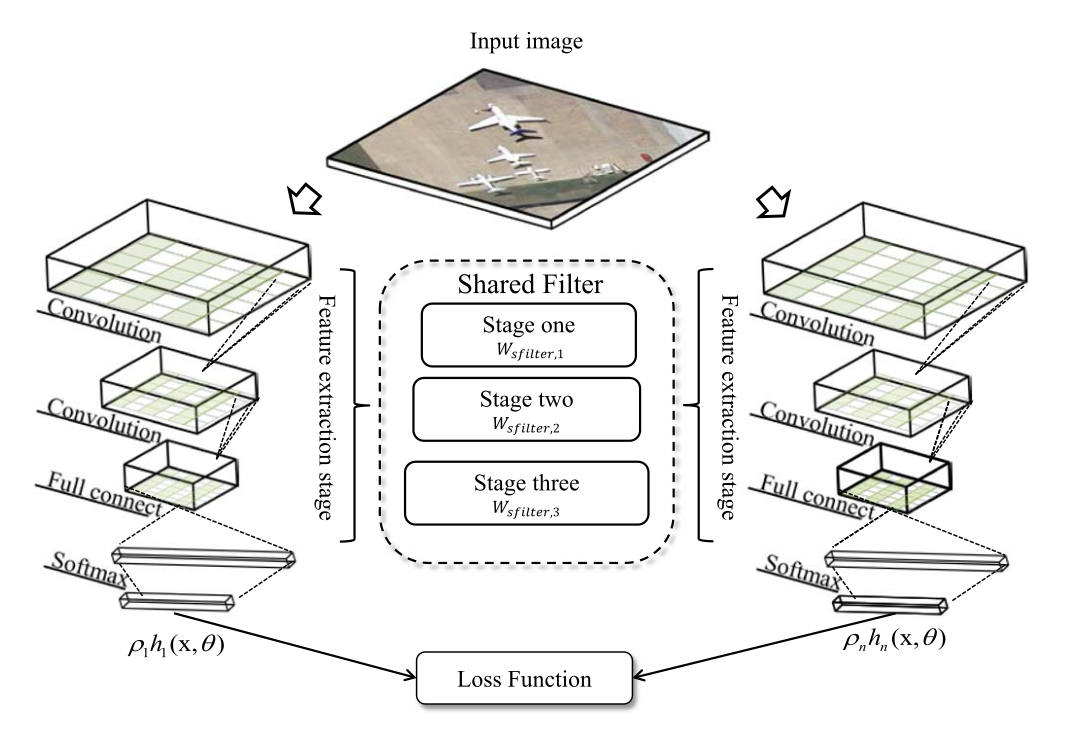
\includegraphics[width=1\linewidth]{images/gbrcnn_architecture}
	\caption[Arquitectura de la red]{Arquitectura de la red}
	\label{fig:gbrcnnarchitecture}
\end{figure}


Durante cada función RCNet se samplea aleatoriamente un set de filtros del banco de filtros compartidos para construir la etapa de extración de características de la RCNet y simultáneamente actualizar los parámetros de la RCNet y el banco de filtros compartido. El tamaño del filtro de del banco de filtros compartidos es mayor al del filtro en la función RCNet de manera que diferentes redes compartirán algunos parámetros. 

Para concluir, los investigadores pusieron a prueba la arquitectura (ver Fig. \ref{fig:gbrcnnarchitecture}) con dos datasets centrados en imágenes satelitales, comparando los resultados con arquitecturas clásicas de clasificación de imágenes y demostrando no sólo que la red propuesta es apropiada como aprendiz base en arquitecturas de ensamblado, sino que también es posible alcanzar el estado del arte y superarlos en relación a los métodos tradicionales.

\subsection{Clasificación de escenas mediante Aprendizaje por Transferencia} \label{ssec:transfer_learning}
En \cite{raahlen2019image}, un trabajo realizado por R{\aa}hl{\'e}n Oskar y Sj{\"o}qvist Sacharias en 2019, se trabajó específicamente con los fines de utilizar el aprendizaje mediante transferencia para clasificar imágenes de propiedades.
Resumidamente, ya que luego se abordará debidamente el tópico en el marco teórico, el aprendizaje mediante transferencia se trata de utilizar una red preentrenada \(R\) con un conjunto de datos \(A\) para resolver un problema relacionado a un dataset \(B\), y la manera para hacerlo es reentrenar la red R con los datos del dataset \(B\). Para este proyecto utilizaron como redes preentrenadas ResNet18, AlexNet, VGG-11, DenseNet-121 e Inception-v3.
Los datos con los que cuentan en esta investigación son imágenes extraídas de Google Image search y \cite{hemnet}, distribuidos de la siguiente manera para cada etiqueta como se observa en la Fig. \ref{fig:transferlearningdataset}.
\begin{figure}[h!]
	\centering
	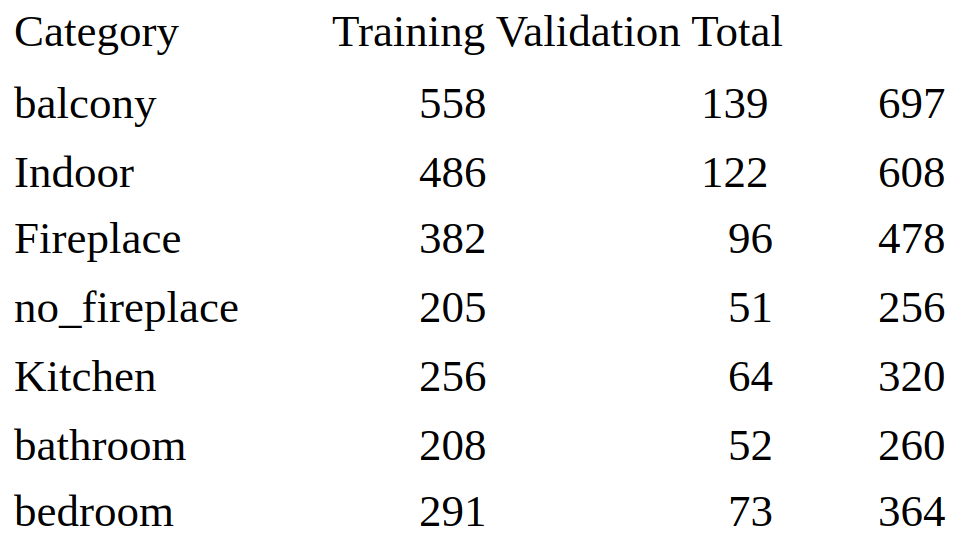
\includegraphics[width=0.7\linewidth]{images/transfer_learning_dataset}
	\caption[Distribución de las imágenes por categoría etiquetada]{Distribución de las imágenes por categoría etiquetada}
	\label{fig:transferlearningdataset}
\end{figure}


En el trabajo se realizaron tres experimentos, y en cada uno de ellos se testearon todas las redes descriptas previamente, con y sin refinamiento de las mismas. El primero se trata de un clasificador binario para predecir si una imagen contiene o no un balcón; el segundo es igualmente un clasificador binario pero que predice si en la imagen se encuentra un hogar (por ejemplo, hogar a leña), y en el tercer experimento plantean una clasificación multiclase en la que intentan etiquetar las imágenes según si se trata de una cocina, un dormitorio o un baño. Es sobre éste último sobre el que se hará énfasis. 
Los experimentos con clasificadores binarios para estimar si se encuentra de un balcón o un hogar a leña en la imagen no resultan de gran interés para este problema, aunque es importante remarcar que para el primero se alcanza una exactitud de un 98\% luego de refinamientos utilizando la red Inception-v3, mientras que para el segundo el mayor porcentaje se alcanza con la red DenseNet y alcanza un 85.5\%. 
El experimento realizado que resulta de mayor importancia para este proyecto es el tercero, un clasificador de múltiples etiquetas que intenta determinar si la imagen se trata de una cocina, un dormitorio o un baño. Las métricas obtenidas antes de realizar refinamiento de las redes testeadas se dan a conocer en la Fig. \ref{fig:metricstransferlearning}
\begin{figure}[h!]
	\centering
	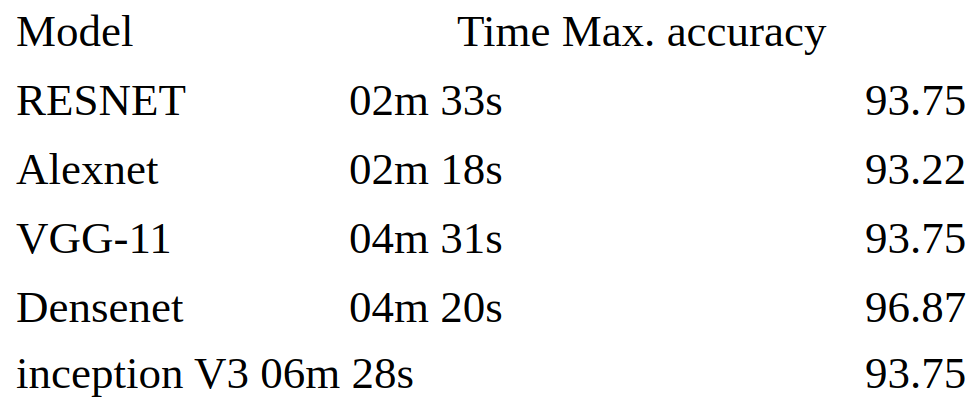
\includegraphics[width=0.6\linewidth]{images/metrics_transfer_learning}
	\caption[metrics_transfer_learning]{Métricas usando extracción de características de los modelos preentrenados}
	\label{fig:metricstransferlearning}
\end{figure}
Luego de hacer refinamiento de las redes entrenando con las imágenes del dataset generado por los investigadores se alcanzan los resultados expuestos en la Fig \ref{fig:metricstransferlearningfinetunned}.

\begin{figure}[h!]
	\centering
	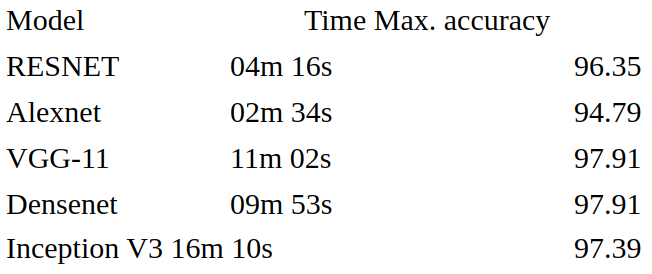
\includegraphics[width=0.7\linewidth]{images/metrics_transfer_learning_fine_tunned}
	\caption[metricstransferlearningfinetunned]{Métricas luego de realizar refinamiento de las redes}
	\label{fig:metricstransferlearningfinetunned}
\end{figure}

Como se puede observar, luego de reentrenar los modelos se obtienen mejoras bastante representativas, dado el percentil de exactitud en que se encuentran los resultados. Otro punto a denotar es que en ambos casos es la red DenseNet la que obtiene la mejor performance, aunque toma aproximadamente el doble que el resto de las redes en entrenarse.
Los autores concluyen su trabajo explicando que a partir de un bajo número de imágenes para su datasets, y a través de aprendizaje por transferencia, es posible agregar palabras claves a las imágenes, como ser: balcón, hogar, baño, cocina y habitación.

\subsection{Otros trabajos relacionados a las propiedades inmuebles que toman provecho de las imágenes de los mismos}

En \cite{vision_based_real_estate_price_estimation} Poursaeed y otros se dedican a la tarea de la estimación de precios de inmuebles basándose en las características visuales de las propiedades. El trabajo incluye una evaluación del impacto visual de las características de una casa en su valor de mercado, la estimación de lujosidad mediante redes neuronales convolucionales, un armazón para la automatización de la valuación utilizando tanto imágenes de las propiedades como metadatos de las mismas y experimentos en los que aplican su trabajo a un nuevo dataset.
Para comenzar se encargaron de obtener alrededor de doscientas mil imágenes correspondientes a diferentes ambientes de casas a partir del dataset Places, Houzz (una empresa de alquiler y venta de viviendas) y búsquedas en Google Imágenes. Luego, entrenaron una red con arquitectura DenseNet para la tarea de predecir las etiquetas baño, dormitorio, cocina, living, comedor, interior y exterior. Con este clasificador, alcanzaron un 91\% de exactitud en el set de test.
A partir de las imágenes etiquedas, en esta investigación propusieron segmentar cada habitación en ocho niveles de lujosidad utilizando la herramienta de crowdsourcing Amazon Mechanical Terk con el fin de obtener estas etiquetas de cada sector. De esta manera, se hicieron de un embedding de baja dimensión en el cual las imágenes con el mismo nivel de lujosidad se encuentran cercanas entre sí. Mediante el algoritmo t-STE los investigadores obtuvieron un embedding bidimensional de las imágenes, que a partir de visualizaciones de los clusters se determinó que las imágenes con mayor nivel de lujosidad quedan en el centro, mientras que las menos lujosas se ubican alrededor. Para aquellas casas que no presentaban imagen de alguno de los ambientes, lo que hicieron fue imputar el promedio de las otras categorías para representar el nivel de lujosidad de ese ambiente.
Una actividad aparte para ellos fue la estimación de precios, para la cual implementaron una regresión que absorve tanto la salida de los modelos que estiman la lujosidad de las habitaciones previamente clasificadas por la DenseNet, como metadatos al respecto de la propiedad (precio de oferta, tamaño, años desde su construcción, cantidad de habitaciones de cada tipo, etc). Vale aclarar que la etiqueta a predecir en cada propiedad es el valor final al que fue adquirida.
\begin{figure}[h!]
	\centering
	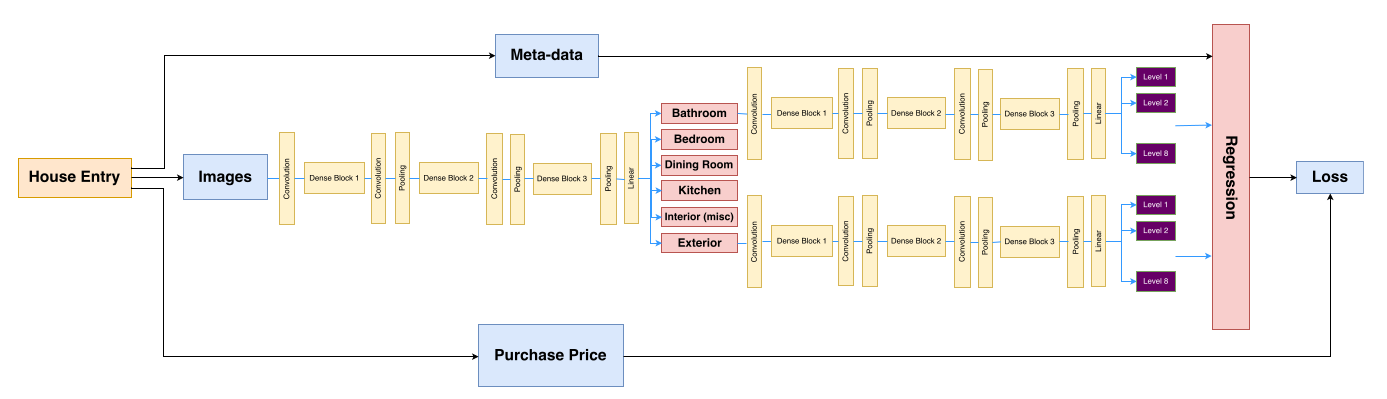
\includegraphics[width=1\linewidth, height=0.35\textheight]{arquitectura_vision_based}
	\caption[Vision Based Architecture]{Arquitectura de la red descripta}
	\label{fig:arquitecturavisionbased}
\end{figure}

Finalmente, con la arquitectura utilizada (ver Fig. 	\ref{fig:arquitecturavisionbased}) demostraron que es posible mejorar los resultados de estimaciones que actualmente se utilizan en el mercado (Índice Zestimate de Zillow) disminuyendo la mediana del error de un 7.9\% a un 5.6\% logrado a partir de la arquitectura presentada.

\subsection{Antecedentes no académicos}
Dentro de los antecedentes que no califican como investigaciones, nos encontramos con \cite{restb_ai}, un proyecto comenzado en 2016 por Angel Esteban. "Buscando entre docenas de propiedades, él estaba shockeado por la inconsistencia en la calidad de las mismas y la dificultad general para encontrar la casa de ensueños para su familia. Tenía que haber una mejor manera." es lo que muestran en la historia de la empresa, que actualmente cuenta con oficinas en Estados Unidos y Europa.
Dentro de las capacidades de visión por computadora que listan relacionadas a las propiedades se encuentran la clasificación de escenas, la detección de características dentro de una imagen, análisis de estado de las habitaciones.
Además, gracias a las capacidades mencionadas anteriormente en su sitio, demuestran cómo se aprovecharon del etiquetado de las imágenes para generar sus productos. Éstos son avocados a la experiencia de usuario, modelos de datos y moderación de contenido. En relación a la experiencia de usuario detallan tres productos fundamentales: la experiencia en búsquedas, el análisis comparativo del mercado y la conversión de imagen a discurso. Por el lado de los modelos de datos se encuentran la valoración automática de propiedades, completar información al respecto de una propiedad que pueda no haber sido detallada, es decir, la integridad de datos, las publicidades dirigidas y la análitica de datos relacionados a este contexto. Por parte de la moderación de contenidos se encuentra la detección de marcas de agua, detección de imágenes duplicadas y la detección de información sensible dentro de la imagen (patentes, números telefónicos, rostros).
Como se puede ver, algunos de estos productos resultan ya definidos como posibles formas de aprovechar el etiquetado de imágenes en la motivación del proyecto, aunque otros no fueron mencionados y también continúan agregando valor y razón de ser a esta investigación.